\newcommand{\pluseq}{\mathrel{+}=}

\newcommand{\familybasedlego}{
	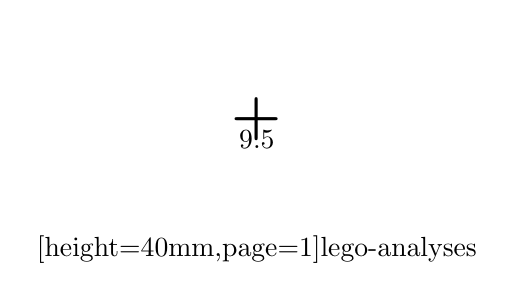
\begin{tikzpicture}
		\node (lego) at (0,-1.7) {\pic[height=40mm,page=1]{lego-analyses}};
		\node (lego) at (0,-.05) {\huge \textbf{+}};
		\node (lego) at (0,1) {\footnotesize\featureDiagramLego};
		\node at (0,-.3) {\mglass{9.5}};
	\end{tikzpicture}
}

\newcommand{\summaryproductbased}{
	\centering\pic[width=.8\linewidth,page=9]{lego-analyses}
	\mynote{Product-Based Strategy}{
		\begin{itemize}
			\item analyze individual \emph{products}
			\item[+] sound, complete
			\item[+] uses off-the-shelf generator\,$\gamma$ and analysis\,$\alpha$
			\item[--] redundant effort
			\item[--] does not scale well
		\end{itemize}
	}
}

\newcommand{\summaryfeaturebased}{
	\centering\pic[width=.8\linewidth,page=6]{lego-analyses}
	\mynote{Feature-Based Strategy}{
		\begin{itemize}
			\item analyze individual \emph{features}
			\item[+] sound, efficient
			\item[--] analysis $\alpha$ requires features with interfaces
			\item[--] incomplete: misses all feature interactions
		\end{itemize}
	}
}

\newcommand{\summaryfamilybased}{
	\centering\scalebox{.5}{\familybasedlego}
	\mynote{Family-Based Strategy}{
		\begin{itemize}
			\item analyze the \emph{product line}
			\item[+] sound, complete, efficient
			\item[--] requires careful, hand-crafted analysis $\alpha$
		\end{itemize}
	}
}

\subsection{Recap: Quality Assurance}

\begin{frame}{\myframetitle\ \mytitlesource{\ludewiglichter}}
	\hfill%
	\only<1|handout:0>{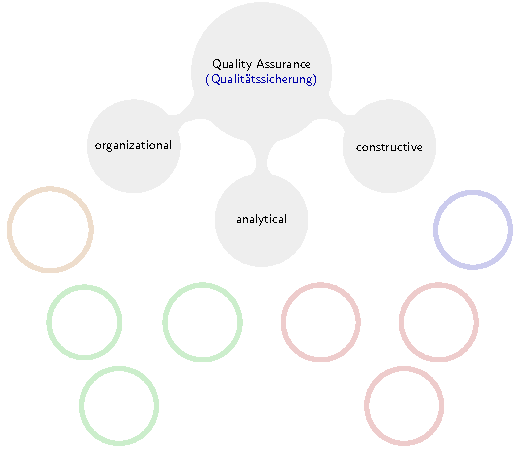
\includegraphics[height=\textheightwithtitle,page=1]{quality-assurance}}%
	\only<2|handout:0>{\includegraphics[height=\textheightwithtitle,page=2]{quality-assurance}}%
	\only<3|handout:0>{\includegraphics[height=\textheightwithtitle,page=3]{quality-assurance}}%
	\only<4|handout:0>{\includegraphics[height=\textheightwithtitle,page=4]{quality-assurance}}%
	\only<5|handout:1>{\includegraphics[height=\textheightwithtitle,page=5]{quality-assurance}}%
	\only<6|handout:0>{\includegraphics[height=\textheightwithtitle,page=6]{quality-assurance}}%
\end{frame}

\begin{frame}{}
	\todo{motivating example that software quality matters, static analysis matters}
\end{frame}

\subsection{Automated Analysis of Product Lines}

%avoiding bugs is nice - finding bugs is also necessary

\begin{frame}{\myframetitle}
	\begin{mycolumns}[t,widths={47}]
		\mynote{Typical Program Analyses}{
			\leftandright{
				\begin{itemize}
					\item code metrics
					\item type checking
					\item theorem proving
					\item data-flow analysis
					\item performance analysis
					\item \ldots
				\end{itemize}
			}{
				\hspace*{10mm}\mglass{3}
			}
		}
		\mydefinition{What is a Program Analysis?}{
			\begin{itemize}
				\item analyzes properties of a \emph{program} (e.g., correctness, performance, and safety)
				\item can be used to automatically find bugs, bottlenecks, and other \emph{vulnerabilities}
			\end{itemize}
		}
		\mynextcolumn
		\myexample{Asking Questions About Product Lines}{
			\begin{itemize}
				\item Which product has the most lines of code? \mysource{\href{https://dl.acm.org/doi/10.1145/3307630.3342384}{ref}}
				\item Which products have type errors? \mysource{\href{https://dl.acm.org/doi/10.1145/1868688.1868693}{ref}}
				\item Which products violate specifications? \mysource{\href{https://dl.acm.org/doi/10.1145/2371401.2371404}{ref}}
				\item Which products have unsafe data flows? \mysource{\href{https://dl.acm.org/doi/10.1145/2499370.2491976}{ref}}
				\item Which is the fastest product? \mysource{\href{https://link.springer.com/article/10.1007/s10515-020-00273-8}{ref}}\\
					Which product has the smallest binary? \mysource{\href{https://dl.acm.org/doi/10.1145/3546932.3546997}{ref}}
				\item \ldots
			\end{itemize}
		}
		\mydefinition{What is a Product-Line Analysis?}{
			\begin{itemize}
				\item analyzes properties of an entire \emph{product line}
				\item can be roughly classified by its \emph{strategy}:
				\begin{itemize}
					\item product-based
					\item feature-based
					\item family-based
				\end{itemize}
			\end{itemize}
		}
	\end{mycolumns}
\end{frame}

\subsection{Product-Based Strategies} % refs missing in whole part!

\begin{frame}{\myframetitle}
	\begin{mycolumns}
		\mydefinition{Intuition}{
			\begin{itemize}
				\item to analyze the product line, just analyze \emph{each product}
				\begin{itemize}
					\item individually
					\item in isolation
					\item possibly in parallel
				\end{itemize}
				\item e.g., compile and verify each product
			\end{itemize}
		}
		\myexampletight{}{\centering\featureDiagramLego\\$Helmet \pimplies \pnot Phone$}
	\mynextcolumn
		\pic[width=\linewidth,page=9]{lego-analyses}
	\end{mycolumns}
\end{frame}

\begin{frame}{\myframetitle}
	\begin{mycolumns}
		\mydefinition{Algorithm}{
			\begin{algorithmic}
				\Require a product line $pl$; algorithms $\gamma$, $\alpha$, $\sigma$
				\State $C \gets AllSAT(\phi(FM_{pl}))$ \Comment{{\small enumerate valid config's}}
				\State $results \gets []$
				\ForAll{$S \in C$} \Comment{{\small for each valid config}}
				\State $p \gets \gamma(S)$ \Comment{{\small generate product}}
				\State $results \pluseq \alpha(p)$ \Comment{{\small add analysis result}}
				\EndFor
				\State \Return $\sigma(results)$
			\end{algorithmic}
		}
		\mynote{}{
			\begin{itemize}
				\item $\gamma$ \emph{generates} (e.g., compiles) products (e.g., \texttt{make}, \texttt{gradle}, \texttt{FeatureHouse}, \texttt{npm}, \ldots)
				\item $\alpha$ \emph{analyzes} the product (e.g., run verifier)
				\item $\sigma$ \emph{summarizes} the results (e.g., each individual call to $\alpha$ must succeed)
			\end{itemize}
		}
	\mynextcolumn
		\myexampletight{}{
			\begin{center}
				\small\featureDiagramConfigurableDatabase
			\end{center}
		}
		\myexample{}{
			\footnotesize
			\leftandright{
				$\sigma([\alpha(\gamma(\{C,G,W\}))$\\
				$~~~~\alpha(\gamma(\{C,P,W\}))$\\
				$~~~~\alpha(\gamma(\{C,G,P,W\}))$\\
				$~~~~\alpha(\gamma(\{C,D,W\}))$\\
				$~~~~\alpha(\gamma(\{C,G,D,W\}))$\\
				$~~~~\alpha(\gamma(\{C,P,D,W\}))$\\
				$~~~~\alpha(\gamma(\{C,G,P,D,W\}))$\\
				$~~~~\alpha(\gamma(\{C,P,T,W\}))$\\
				$~~~~\alpha(\gamma(\{C,G,P,T,W\}))$\\
				$~~~~\alpha(\gamma(\{C,D,T,W\}))$\\
				$~~~~\alpha(\gamma(\{C,G,D,T,W\}))$\\
				$~~~~\alpha(\gamma(\{C,P,D,T,W\}))$\\
				$~~~~\alpha(\gamma(\{C,G,P,D,T,W\}))$
			}{
				$\alpha(\gamma(\{C,G,L\}))$\\
				$\alpha(\gamma(\{C,P,L\}))$\\
				$\alpha(\gamma(\{C,G,P,L\}))$\\
				$\alpha(\gamma(\{C,D,L\}))$\\
				$\alpha(\gamma(\{C,G,D,L\}))$\\
				$\alpha(\gamma(\{C,P,D,L\}))$\\
				$\alpha(\gamma(\{C,G,P,D,L\}))$\\
				$\alpha(\gamma(\{C,P,T,L\}))$\\
				$\alpha(\gamma(\{C,G,P,T,L\}))$\\
				$\alpha(\gamma(\{C,D,T,L\}))$\\
				$\alpha(\gamma(\{C,G,D,T,L\}))$\\
				$\alpha(\gamma(\{C,P,D,T,L\}))$\\
				$\alpha(\gamma(\{C,G,P,D,T,L\}))])$
			}
		}
	\end{mycolumns}
\end{frame}

\begin{frame}{Classification of Strategies}
	\begin{mycolumns}[t,columns=3]
		\summaryproductbased
	\mynextcolumn
	\mynextcolumn
	\end{mycolumns}
\end{frame}

\subsection{Feature-Based Strategies}

\begin{frame}{\myframetitle}
	\begin{mycolumns}
		\mydefinition{Intuition}{
			\begin{itemize}
				\item to analyze the product line, just analyze \emph{each feature} individually
				\item ignore all relations to other features
				\item e.g., compile and verify each component\\
				$\Rightarrow$ requires \emph{interfaces between features} (components, services, plug-ins) % todo: rename lecture 6 accordingly?
			\end{itemize}
		}
		\myexampletight{}{\centering\featureDiagramLego\\$Helmet \pimplies \pnot Phone$}
	\mynextcolumn
		\pic[width=\linewidth,page=6]{lego-analyses}
	\end{mycolumns}
\end{frame}

\begin{frame}{\myframetitle}
	\begin{mycolumns}
		\mydefinition{Algorithm}{
			\begin{algorithmic}
				\Require a product line $pl$; algorithms $\alpha$, $\sigma$
				\State $results \gets []$
				\ForAll{$f \in F_{pl}$} \Comment{{\small for each feature}}
				\State $results \pluseq \alpha(f)$ \Comment{{\small add analysis result}}
				\EndFor
				\State \Return $\sigma(results)$
			\end{algorithmic}
		}
		\mynote{}{
			\begin{itemize}
				\item $\alpha$ \emph{analyzes} the feature (e.g., compiles and verifies the component)
				\item $\sigma$ \emph{summarizes} the results (see product-based)
			\end{itemize}
		}
	\mynextcolumn
		\myexampletight{}{
			\begin{center}
				\small\featureDiagramConfigurableDatabase
			\end{center}
		}
		\myexample{}{
			\vspace*{-4ex}
			\small
			\begin{align*}
				\sigma([&\alpha(\gamma(C)) \text{ -- e.g., compile and verify base code}\\
				&\alpha(\gamma(G)) \text{ -- e.g., compile and verify feature Get}\\
				&\alpha(\gamma(P)) \text{ -- \ldots}\\
				&\alpha(\gamma(D))\\
				&\alpha(\gamma(T))\\
				&\alpha(\gamma(W))\\
				&\alpha(\gamma(L))])
			\end{align*}
		}
	\end{mycolumns}
\end{frame}

\begin{frame}{Classification of Strategies}
	\begin{mycolumns}[t,columns=3]
		\summaryproductbased
	\mynextcolumn
		\summaryfeaturebased
	\mynextcolumn
	\end{mycolumns}
\end{frame}

\subsection{Family-Based Strategies}

\begin{frame}{\myframetitle}
	\begin{mycolumns}
		\mydefinition{Intuition}{
			\begin{itemize}
				\item analyze the product line (or \emph{family}) as a whole
				\item requirement: the analysis should give the same result as a product-based analysis
				\item makes use of the feature model and artifacts
				\item analysis is \emph{hand-crafted}, no generic algorithm\\
				$\Rightarrow$ typically: reduction to SAT problems
			\end{itemize}
		}
		\myexample{Today's Examples}{
			\begin{itemize}
				\item analyzing \emph{feature mappings}
				\item analyzing \emph{variable code}
			\end{itemize}
			$\Rightarrow$ here: only for \emph{conditional compilation}
		}
	\mynextcolumn
		\centering\familybasedlego
	\end{mycolumns}
\end{frame}

\subsection{Classification of Strategies}

\begin{frame}{\myframetitle}
	\begin{mycolumns}[t,columns=3]
		\summaryproductbased
	\mynextcolumn
		\summaryfeaturebased
	\mynextcolumn
		\summaryfamilybased
	\end{mycolumns}
\end{frame}